\chapter{HASIL DAN UJI COBA}
\tab Pada bab ini akan dipaparkan hasil uji coba saat sistem dijalankan. Uji coba sistem \textit{Monitoring} SIK akan dilakukan untuk memastikan kualitas perangkat lunak yang dikembangkan dengan analisis dan perancangan perangkat lunak.

\section{Lingkungan Uji Coba}
Lingkungan uji coba sistem pada Kerja Praktik kali ini meliputi perangkat keras dan perangkat lunak adalah sebagai berikut:
\begin{enumerate}
\item Perangkat Keras
	\begin{enumerate}
	\item \textit{Processor} Intel(R) Core i3-330M @ 2.13 GHz
	\item Memori 4GB
	\end{enumerate}
\item Perangkat Lunak
	\begin{enumerate}
	\item Sistem Operasi Windows 10 64 bit
	\end{enumerate}
\end{enumerate}

\section{Skenario Pengujian}
Skenario pengujian yang akan dilakukan pada aplikasi \textit{Monitoring} SIK adalah melakukan peran sebagai admin yang sedang membuka aplikasi. Langkah-langkah dari skenario adalah sebagai berikut:
	\begin{enumerate}
	\item User membuka aplikasi \textit{Monitoring} SIK.
	\item User memilih menu \textit{request} relokasi, SIK, eksekusi, penagihan dan finish.
	\item User menambahkan data \textit{request} relokasi dan SIK dengan mengisi \textit{form}.
	\item User melihat detail \textit{request} relokasi, SIK, eksekusi, penagihan dan finish.
	\end{enumerate}
\subsection{Pengujian Menampilkan Data \textit{Request} Relokasi}
Pengujian ini dilakukan terhadap fungsionalitas menampilkan data \textit{request} relokasi. Tabel \ref{tab:list_req_relokasi} menjelaskan pengujian fungsionalitas ini. Gambar \ref{figure:data_req_relokasi} adalah hasil fungsionalitas menampilkan data \textit{request} relokasi.

\begin{table}[h!]
	\centering
	\begin{tabular}{|p{4cm}|p{6cm}|}
	\hline
	Kode \textit{Use Case} & UC-001\\ \hline
	Tujuan Pengujian & Menampilkan semua data \textit{request} relokasi\\ \hline
	Data Masukan & - \\ \hline
	Prosedur Pengujian & 
		\begin{enumerate}
		\item Pengguna \textit{login} sebagai administrator
		\item Pengguna memilih menu \textit{request} relokasi
		\end{enumerate}\\ \hline
	Hasil yang diharapkan & Semua data \textit{request} relokasi dapat ditampilkan pada menu \textit{request} relokasi dan dapat dipilih untuk melihat detailnya \\ \hline
	Hasil yang diperoleh & Semua data \textit{request} relokasi dapat ditampilkan pada menu \textit{request} relokasi dan detailnya dapat ditampilkan\\ \hline
	Kesimpulan & Proses menampilkan data \textit{request} relokasi beserta detailnya berhasil\\ \hline
	Kondisi Akhir & Pengguna mendapatkan semua informasi data \textit{request} relokasi\\ \hline
	\end{tabular}\caption{Skenario Pengujian Menampilkan Data \textit{Request} Relokasi}
	\label{tab:list_req_relokasi}
\end{table}

\begin{figure}[h!]
\centerline
{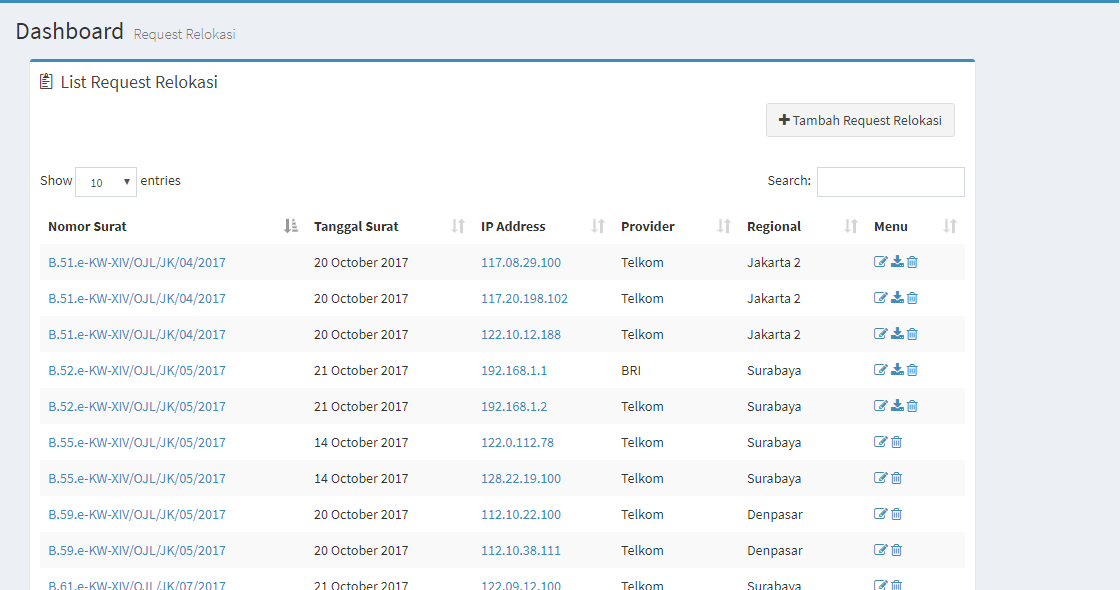
\includegraphics[width=10cm,height=5cm]{bab6/listReqRelokasi.png}}
\caption{Data \textit{Request} Relokasi}
\label{figure:data_req_relokasi}
\end{figure}

\subsection{Pengujian Menampilkan Data SIK}
Pengujian ini dilakukan terhadap fungsionalitas menampilkan data SIK. Tabel \ref{tab:list_sik} menjelaskan pengujian fungsionalitas ini. Gambar \ref{figure:data_detail_sik} adalah hasil fungsionalitas menampilkan data SIK.
\begin{figure}[h!]
\centerline
{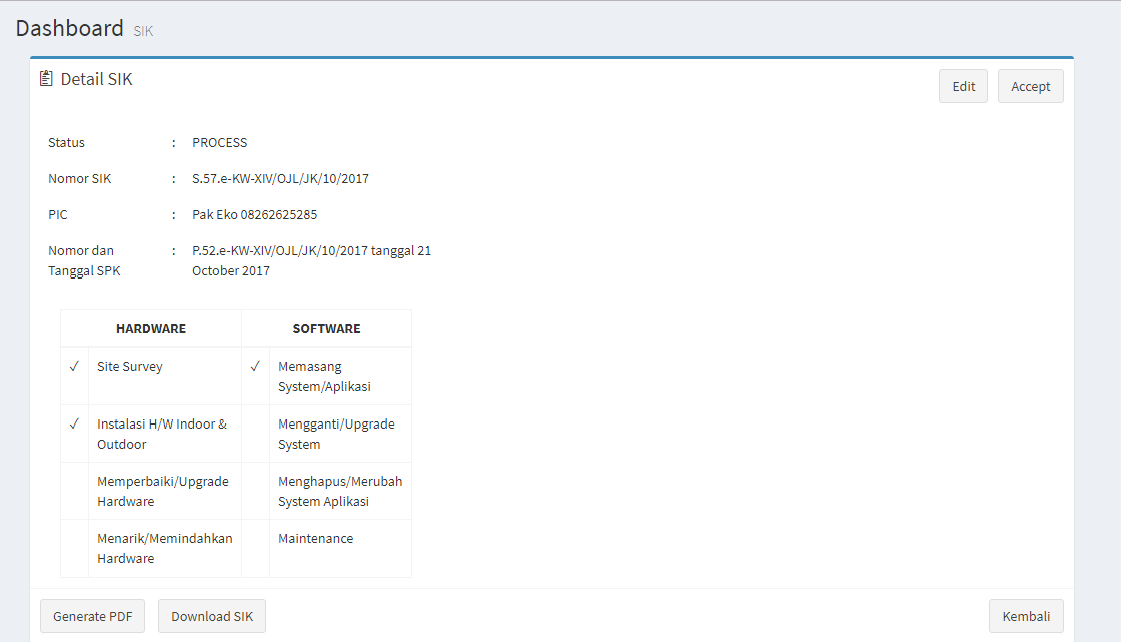
\includegraphics[width=10cm,height=5cm]{bab6/detailSIK.png}}
\caption{Data Detail SIK}
\label{figure:data_detail_sik}
\end{figure}

\begin{table}[h!]
	\centering
	\begin{tabular}{|p{4cm}|p{6cm}|}
	\hline
	Kode \textit{Use Case} & UC-002\\ \hline
	Tujuan Pengujian & Menampilkan semua data SIK\\ \hline
	Data Masukan & - \\ \hline
	Prosedur Pengujian & 
		\begin{enumerate}
		\item Pengguna \textit{login} sebagai administrator
		\item Pengguna memilih menu SIK
		\end{enumerate}\\ \hline
	Hasil yang diharapkan & Semua data SIK dapat ditampilkan pada menu SIK dan dapat dipilih untuk melihat detailnya \\ \hline
	Hasil yang diperoleh & Semua data SIK dapat ditampilkan pada menu SIK dan detailnya dapat ditampilkan\\ \hline
	Kesimpulan & Proses menampilkan data SIK beserta detailnya berhasil\\ \hline
	Kondisi Akhir & Pengguna mendapatkan semua informasi data SIK\\ \hline
	\end{tabular}\caption{Skenario Pengujian Menampilkan Data SIK}
	\label{tab:list_sik}
\end{table}

\subsection{Pengujian Menampilkan Data Eksekusi}
Pengujian ini dilakukan terhadap fungsionalitas menampilkan data Eksekusi. Tabel \ref{tab:list_eksekusi_1} dan \ref{tab:list_eksekusi_2} menjelaskan pengujian fungsionalitas ini. Gambar \ref{figure:data_detail_eksekusi} adalah hasil fungsionalitas menampilkan data Eksekusi.

\begin{table}[h!]
	\centering
	\begin{tabular}{|p{4cm}|p{6cm}|}
	\hline
	Kode \textit{Use Case} & UC-003\\ \hline
	Tujuan Pengujian & Menampilkan semua data Eksekusi\\ \hline
	Data Masukan & - \\ \hline
	\end{tabular}\caption{Skenario Pengujian Menampilkan Data Eksekusi(1)}
	\label{tab:list_eksekusi_1}
\end{table}

\begin{table}[h!]
	\centering
	\begin{tabular}{|p{4cm}|p{6cm}|}
	\hline
	Prosedur Pengujian & 
		\begin{enumerate}
		\item Pengguna \textit{login} sebagai administrator
		\item Pengguna memilih menu Eksekusi
		\end{enumerate}\\ \hline
	Hasil yang diharapkan & Semua data Eksekusi dapat ditampilkan pada menu Eksekusi dan dapat dipilih untuk melihat detailnya \\ \hline
	Hasil yang diperoleh & Semua data Eksekusi dapat ditampilkan pada menu Eksekusi dan detailnya dapat ditampilkan\\ \hline
	Kesimpulan & Proses menampilkan data Eksekusi beserta detailnya berhasil\\ \hline
	Kondisi Akhir & Pengguna mendapatkan semua informasi data Eksekusi\\ \hline
	\end{tabular}\caption{Skenario Pengujian Menampilkan Data Eksekusi(2)}
		\label{tab:list_eksekusi_2}
\end{table}

\begin{figure}[h!]
\centerline
{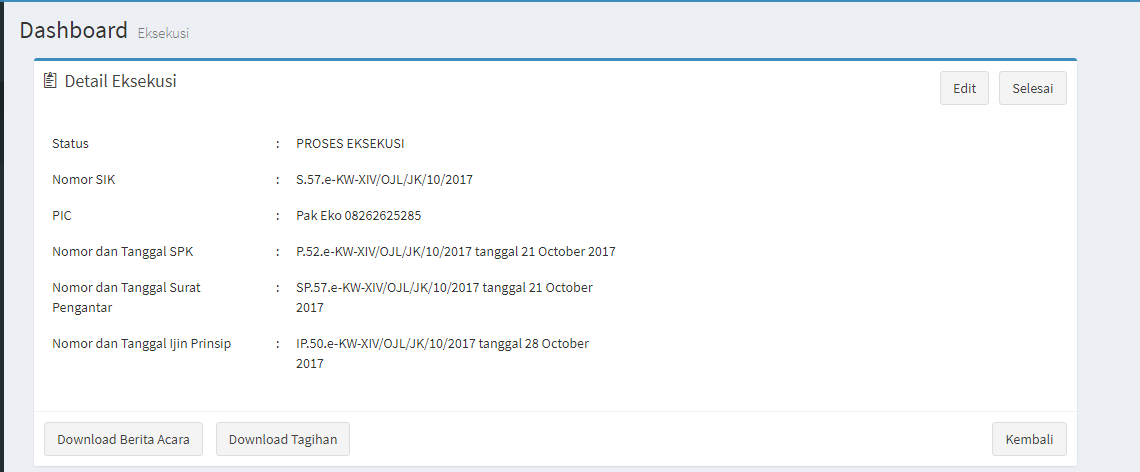
\includegraphics[width=10cm,height=5cm]{bab6/detailExecution.png}}
\caption{Data Detail Eksekusi}
\label{figure:data_detail_eksekusi}
\end{figure}

\subsection{Pengujian Menampilkan Data Penagihan}
Pengujian ini dilakukan terhadap fungsionalitas menampilkan data Penagihan. Tabel \ref{tab:list_penagihan_1} dan \ref{tab:list_penagihan_2} menjelaskan pengujian fungsionalitas ini. Gambar \ref{figure:data_detail_penagihan} adalah hasil fungsionalitas menampilkan data penagihan.
\begin{figure}[h!]
\centerline
{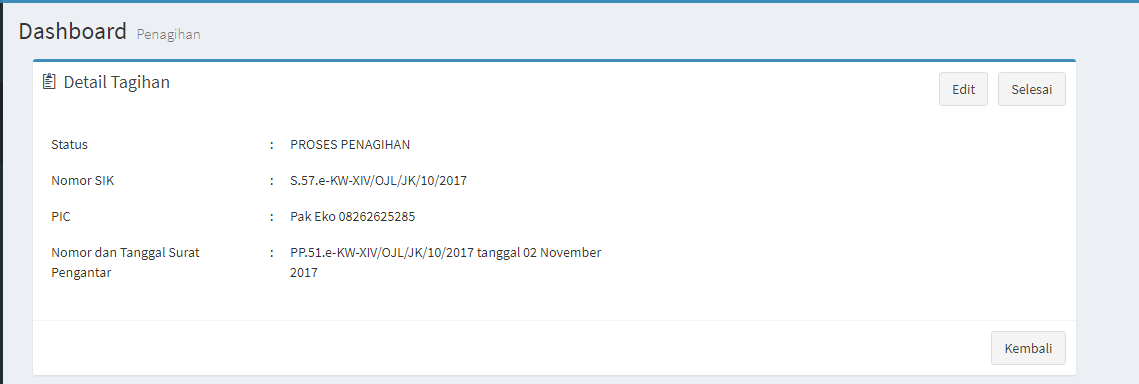
\includegraphics[width=10cm,height=4.5cm]{bab6/detailPenagihan.png}}
\caption{Data Detail Penagihan}
\label{figure:data_detail_penagihan}
\end{figure}

\begin{table}[h!]
	\centering
	\begin{tabular}{|p{4cm}|p{6cm}|}
	\hline
	Kode \textit{Use Case} & UC-004\\ \hline
	Tujuan Pengujian & Menampilkan semua data Penagihan\\ \hline
	Data Masukan & - \\ \hline
	Prosedur Pengujian & 
		\begin{enumerate}
		\item Pengguna \textit{login} sebagai administrator
		\item Pengguna memilih menu Penagihan
		\end{enumerate}\\ \hline
	\end{tabular}\caption{Skenario Pengujian Menampilkan Data Penagihan(1)}
	\label{tab:list_penagihan_1}
\end{table}

\begin{table}[h!]
	\centering
	\begin{tabular}{|p{4cm}|p{6cm}|}
	\hline
	Hasil yang diharapkan & Semua data Penagihan dapat ditampilkan pada menu Penagihan dan dapat dipilih untuk melihat detailnya \\ \hline
	Hasil yang diperoleh & Semua data Penagihan dapat ditampilkan pada menu Penagihan dan detailnya dapat ditampilkan\\ \hline
	Kesimpulan & Proses menampilkan data Penagihan beserta detailnya berhasil\\ \hline
	Kondisi Akhir & Pengguna mendapatkan semua informasi data Penagihan\\ \hline
	\end{tabular}\caption{Skenario Pengujian Menampilkan Data Penagihan(2)}
		\label{tab:list_penagihan_2}
\end{table}

\subsection{Pengujian Menampilkan Data \textit{Finish}}
Pengujian ini dilakukan terhadap fungsionalitas menampilkan data \textit{Finish}. Tabel \ref{tab:list_finish} menjelaskan pengujian fungsionalitas ini. Gambar \ref{figure:data_detail_finish} adalah hasil fungsionalitas menampilkan data \textit{finish}.

\begin{table}[h!]
	\centering
	\begin{tabular}{|p{4cm}|p{6cm}|}
	\hline
	Kode \textit{Use Case} & UC-005\\ \hline
	Tujuan Pengujian & Menampilkan semua data \textit{Finish}\\ \hline
	Data Masukan & - \\ \hline
	Prosedur Pengujian & 
		\begin{enumerate}
		\item Pengguna \textit{login} sebagai administrator
		\item Pengguna memilih menu \textit{Finish}
		\end{enumerate}\\ \hline
	Hasil yang diharapkan & Semua data \textit{Finish} dapat ditampilkan pada menu \textit{Finish} dan dapat dipilih untuk melihat detailnya \\ \hline
	Hasil yang diperoleh & Semua data \textit{Finish} dapat ditampilkan pada menu \textit{Finish} dan detailnya dapat ditampilkan\\ \hline
	Kesimpulan & Proses menampilkan data \textit{Finish} beserta detailnya berhasil\\ \hline
	Kesimpulan & Proses menampilkan data \textit{Finish} beserta detailnya berhasil\\ \hline
	Kondisi Akhir & Pengguna mendapatkan semua informasi data \textit{Finish}\\ \hline
	\end{tabular}\caption{Skenario Pengujian Menampilkan Data \textit{Finish}}
	\label{tab:list_finish}
\end{table}

\begin{figure}[h!]
\centerline
{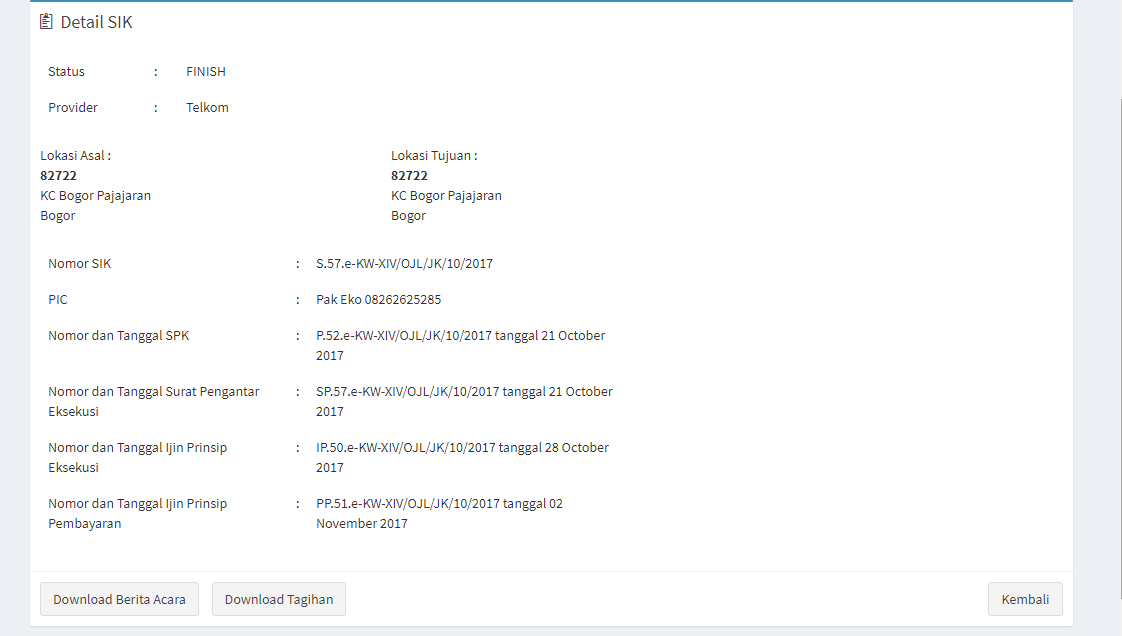
\includegraphics[width=10cm,height=5cm]{bab6/finish.png}}
\caption{Data Detail \textit{Finish}}
\label{figure:data_detail_finish}
\end{figure}

\section{Evaluasi Pengujian}
\tab Hasil pengujian dihasilkan pengamatan lebih lanjut terhadap perilaku sistem \textit{Monitoring} SIK terhadap skenario kasus uji coba. Pengujian dilakukan \textit{internal team} untuk mencoba sistem yang telah diterapkan. Tabel \ref{tab:hasil_pengujian} adalah hasil pengujian pada sistem informasi \textit{monitoring} SIK.
\begin{table}[h!]
	\centering
	\begin{tabular}{|p{6cm}|p{4cm}|}
	\hline
	\textbf{Tugas} & \textbf{Hasil}\\ \hline
	Sistem mampu menampilkan informasi fitur-fitur \textit{Monitoring} SIK & Terpenuhi\\ \hline
	Sistem mampu menampilkan detail informasi kepada user & Terpenuhi\\ \hline
	Sistem mampu menangani pengelolaan data \textit{Monitoring} SIK & Terpenuhi\\ \hline
	Sistem mampu mengeksport data SIK ke dalam bentuk file berekstensi pdf & Terpenuhi\\ \hline
	Sistem menampilkan data sesuai dengan \textit{keyword} pencarian & Terpenuhi\\ \hline
	Sistem dapat mendownload dan upload file ke dalam basis data & Terpenuhi\\ \hline
	\end{tabular}\caption{Hasil Pengujian}
		\label{tab:hasil_pengujian}
\end{table}

Dengan hasil pengujian yang telah dilakukan, dapat disimpulkan bahwa keseluruhan aplikasi \textit{Monitoring} SIK memenuhi kriteria yang disebutkan pada sub-bab sebelumnya.

\section{Evaluasi Performa}
Tabel \ref{tab:evaluasi_performa_1} dan \ref{tab:evaluasi_performa_2} adalah hasil dari uji coba evaluasi performa sistem informasi \textit{monitoring} SIK.
\begin{table}
\centering
\begin{tabular}{|p{5cm}|p{2.5cm}|p{2cm}|}
\hline
\textbf{Tugas} & \textbf{Hasil} & \textbf{Waktu}\\ \hline
Membuka Halaman Dashboard & Terpenuhi & 2 detik\\ \hline
Membuka Halaman Request Relokasi & Terpenuhi & 1 detik\\ \hline
Menambahkan Request Relokasi & Terpenuhi & 2 detik\\ \hline
\end{tabular}\caption{Hasil Uji Performa(1)}
		\label{tab:evaluasi_performa_1}
\end{table}

\begin{table}
\centering
\begin{tabular}{|p{5cm}|p{2.5cm}|p{2cm}|}
\hline
\textbf{Tugas} & \textbf{Hasil} & \textbf{Waktu}\\ \hline
Membuka Halaman SIK & Terpenuhi & 1 detik\\ \hline
Menambahkan SIK & Terpenuhi & 2 detik\\ \hline
Membuka Halaman Penagihan & Terpenuhi & 1 detik\\ \hline
Menambahkan Penagihan & Terpenuhi & 2 detik\\ \hline
Membuka Halaman Eksekusi & Terpenuhi & 1 detik\\ \hline
Menambahkan Eksekusi & Terpenuhi & 2 detik\\ \hline
Membuka Halaman Finish & Terpenuhi & 1 detik\\ \hline
Menambahkan Finish & Terpenuhi & 2 detik\\ \hline
Mendownload Request Relokasi & Terpenuhi & 2 detik\\ \hline
Mendownload SIK & Terpenuhi & 2 detik\\ \hline
Mendownload Berita Acara & Terpenuhi & 2 detik\\ \hline
Mendownload Penagihan & Terpenuhi & 2 detik\\ \hline
\end{tabular}\caption{Hasil Uji Performa(2)}
		\label{tab:evaluasi_performa_2}
\end{table}

\vspace{4 cm}
\textcolor{white}{..}